\documentclass[11pt, letterpaper]{article}

% Packages
\usepackage[margin=1in]{geometry}
\usepackage{graphicx}
\usepackage{amsmath}
\usepackage{amssymb}
\usepackage{booktabs}
\usepackage{hyperref}
\usepackage{float}
\usepackage{caption}
\usepackage{subcaption}
\usepackage{setspace}
\usepackage{titlesec}
\usepackage{fancyhdr}

% Formatting
\onehalfspacing
\setlength{\parskip}{0.5em}
\setlength{\parindent}{0pt}

% Header/Footer
\pagestyle{fancy}
\fancyhf{}
\fancyhead[L]{Fixed Income Allocation Strategy}
\fancyhead[R]{Regentfund Project}
\fancyfoot[C]{\thepage}

% Section formatting
\titleformat{\section}{\Large\bfseries}{\thesection}{1em}{}
\titleformat{\subsection}{\large\bfseries}{\thesubsection}{1em}{}

% Hyperlink colors
\hypersetup{
    colorlinks=true,
    linkcolor=blue,
    citecolor=blue,
    urlcolor=blue
}

\begin{document}

% Title Page
\begin{titlepage}
    \centering
    \vspace*{2cm}

    {\Huge\bfseries Fixed Income Allocation Strategy\par}
    \vspace{0.5cm}
    {\Large Regentfund Project\par}
    \vspace{2cm}

    {\Large\itshape Taiya Shiva\par}
    \vspace{0.5cm}
    {\large Hawk Center for Investment Analysis\par}
    \vspace{2cm}

    {\large \today\par}

    \vfill

    {\small
    Prepared for the Regentfund Fixed Income Portfolio\\
    Hawk Center for Investment Analysis
    \par}

\end{titlepage}

% Abstract
\begin{abstract}
This whitepaper presents a momentum-based tactical asset allocation framework for the Regentfund Fixed Income Portfolio, allocating across high yield (H5A4), investment grade (C5A0), and government bonds (G5O2). The strategy employs blended momentum (BMOM) signals combining 20, 60, 120, and 240-day lookbacks, with 70\% weight on intermediate horizons aligned to credit cycle frequencies. Strategy 1 generates binary long/flat signals through cross-asset benchmark filtering and 240-day trend confirmation, achieving asset-level Sharpe ratios of 0.18--0.28. Strategy 2 introduces a drawdown differential override that locks positions long when tactical signals outperform buy-and-hold by more than 10 percentage points, improving C5A0 performance by 61\% (Sharpe 0.18 to 0.29). Proportional linear allocation weights assets by momentum strength subject to a 12\% high yield cap and 5\% minimum positions, with defensive positioning (10\% cash, 90\% government) when all signals turn flat. The final Monthly Strategy adapts the framework to Regentfund's monthly trading constraint through dual-trigger rebalancing: scheduled monthly execution plus risk-triggered overrides when any signal exits. The implementable strategy achieves a 0.26 Sharpe ratio with 0.77\% annualized return and $-11.99\%$ maximum drawdown, providing systematic tactical allocation with explicit risk management while meeting institutional operational requirements.
\end{abstract}

\newpage
\tableofcontents
\newpage

% Main Content
\section{Introduction}

Fixed income markets exhibit time-varying risk premia that can be systematically captured through momentum-based strategies. This whitepaper presents a quantitative tactical allocation framework developed for the Regentfund Fixed Income Portfolio, managed under the Hawk Center for Investment Analysis. The strategy addresses the need for a systematic, rules-based approach to fixed income allocation that can adapt to changing market conditions while respecting practical portfolio management constraints.

\textbf{Asset Universe}

The strategy allocates across three primary fixed income asset classes:
\begin{itemize}
    \item \textbf{H5A4 (High Yield)}: ICE BofA US High Yield Index tracking U.S. dollar-denominated, non-investment-grade corporate bonds with higher credit risk and return potential
    \item \textbf{C5A0 (Investment Grade)}: ICE BofA US Investment Grade Corporate Index tracking investment-grade rated corporate debt with moderate credit risk
    \item \textbf{G5O2 (Government)}: ICE BofA US Treasury Index tracking fixed-rate U.S. Treasury bonds as a defensive anchor
    \item \textbf{Cash}: Maintained as a buffer (5--10\%) depending on market conditions
\end{itemize}

Performance is benchmarked against Regentfund's baseline static allocation: 66.5\% Investment Grade (C5A0), 9.5\% High Yield (H5A4), 19.5\% Government (G5O2), and 5.0\% Cash. This equal-weight benchmark represents the passive allocation strategy that the tactical framework seeks to outperform.

\textbf{Strategic Approach}

The framework employs a momentum-based signal generation methodology using blended momentum (BMOM) indicators across multiple time horizons (20, 60, 120, and 240-day lookbacks). These signals are combined with cross-asset benchmark filtering to identify periods of momentum deterioration across credit and duration factors. The allocation mechanism uses proportional linear weighting, where stronger momentum signals receive larger portfolio allocations, enabling dynamic risk adjustment based on market conditions.

\textbf{Fixed Income Momentum Dynamics}

Momentum strategies in fixed income markets capture distinct dynamics compared to equity markets. Bond prices mechanically respond to changes in yields, credit spreads, and interest rate expectations through well-defined duration and convexity relationships. Credit spreads (the compensation investors demand for default risk) tend to widen or tighten gradually as economic conditions evolve, creating persistent price trends. Similarly, interest rate regimes exhibit persistence due to central bank policy cycles and the slow-moving nature of macroeconomic fundamentals. These characteristics make momentum particularly relevant for fixed income: rather than exploiting behavioral inefficiencies, momentum signals capture the systematic adjustment of bond prices to changes in fundamental risk factors. The multi-horizon BMOM framework specifically targets these dynamics, with 60-120 day lookbacks aligned to credit cycle frequencies and 240-day lookbacks confirming longer-term interest rate regime shifts.

\textbf{Implementation Constraints}

Two critical constraints shape the final implementation:
\begin{enumerate}
    \item \textbf{High Yield Cap}: Maximum 12\% allocation to H5A4 (high yield) to limit credit concentration risk in the Regentfund portfolio
    \item \textbf{Monthly Rebalancing}: Transaction execution limited to month-end to minimize implementation costs, with exceptions for immediate risk-off signals
\end{enumerate}

\textbf{Strategy Evolution}

This whitepaper documents the research process that led to the final Monthly Rebalancing Strategy through four developmental stages:
\begin{itemize}
    \item \textbf{Strategy 1}: Establishes cross-asset momentum signals with benchmark filtering and long-term trend confirmation
    \item \textbf{Strategy 2}: Introduces drawdown differential override logic to capitalize on periods when tactical signals successfully avoid losses
    \item \textbf{Strategy 3}: Implements proportional linear allocation across all three assets with portfolio constraints and turnover filtering
    \item \textbf{Monthly Strategy}: Optimizes transaction timing through scheduled monthly rebalancing with risk-triggered overrides
\end{itemize}

The following sections detail each component's methodology, implementation logic, and performance characteristics.

\newpage
\section{Methodology}

\subsection{Signal Generation: Blended Momentum (BMOM)}

The foundation of the strategy is a blended momentum (BMOM) indicator that combines price momentum across four distinct time horizons. For each asset $i$ at time $t$, the BMOM signal is calculated as:

\begin{equation}
\text{BMOM}_i(t) = 0.15 \cdot \text{Mom}_{i,20} + 0.35 \cdot \text{Mom}_{i,60} + 0.35 \cdot \text{Mom}_{i,120} + 0.15 \cdot \text{Mom}_{i,240}
\end{equation}

where $\text{Mom}_{i,n}$ represents the $n$-day momentum for asset $i$.

The asymmetric weighting scheme reflects the distinct dynamics captured by each lookback period. The 60-day and 120-day lookbacks receive the highest combined weight (70\%) as these horizons align with typical credit cycle frequencies and capture the gradual widening or tightening of credit spreads as economic conditions evolve. The 20-day lookback (15\% weight) provides tactical responsiveness to recent price action, while the 240-day lookback (15\% weight) serves as a regime confirmation signal, ensuring alignment with longer-term interest rate trends. This weighting structure balances responsiveness to changing market conditions with stability, avoiding overreaction to short-term noise while remaining sensitive to persistent credit and duration dynamics.

\subsection{Strategy 1: Cross-Asset Momentum with Benchmark Filter}

Strategy 1 generates binary signals (long or flat) for each asset independently by combining asset-level BMOM with cross-asset benchmark filtering. This approach uses equity market momentum (SPY) as a universal benchmark filter, exploiting the equity-credit lead-lag relationship to identify periods of systemic risk-off sentiment.

\textbf{Benchmark Pairing}

All three fixed income assets use SPY (equity market) as the universal benchmark for cross-asset momentum confirmation:
\begin{itemize}
    \item \textbf{H5A4 (High Yield)} $\rightarrow$ SPY
    \item \textbf{C5A0 (Investment Grade)} $\rightarrow$ SPY
    \item \textbf{G5O2 (Government)} $\rightarrow$ SPY
\end{itemize}

\textbf{Signal Logic}

For each asset, the strategy employs the following rules:

\textbf{Exit Condition (Signal = 0):} The strategy exits to cash when either cross-below condition is met AND the 240-day momentum is negative:

\begin{align}
C_1 &: \text{BMOM}_{\text{bench}}(t-1) > -0.03 \land \text{BMOM}_{\text{bench}}(t) < -0.03 \land \text{BMOM}_{\text{asset}}(t) < -0.03 \\
C_2 &: \text{BMOM}_{\text{asset}}(t-1) > -0.03 \land \text{BMOM}_{\text{asset}}(t) < -0.03 \land \text{BMOM}_{\text{bench}}(t) < -0.03
\end{align}

Exit if: $(C_1 \lor C_2) \land \text{Mom}_{240} < 0$

\textbf{Entry Condition (Signal = 1):} $\text{BMOM}_{\text{asset}}(t) > 0$

\textbf{Hold:} If neither exit nor entry conditions are met, the strategy maintains its previous signal state.

\begin{figure}[H]
    \centering
    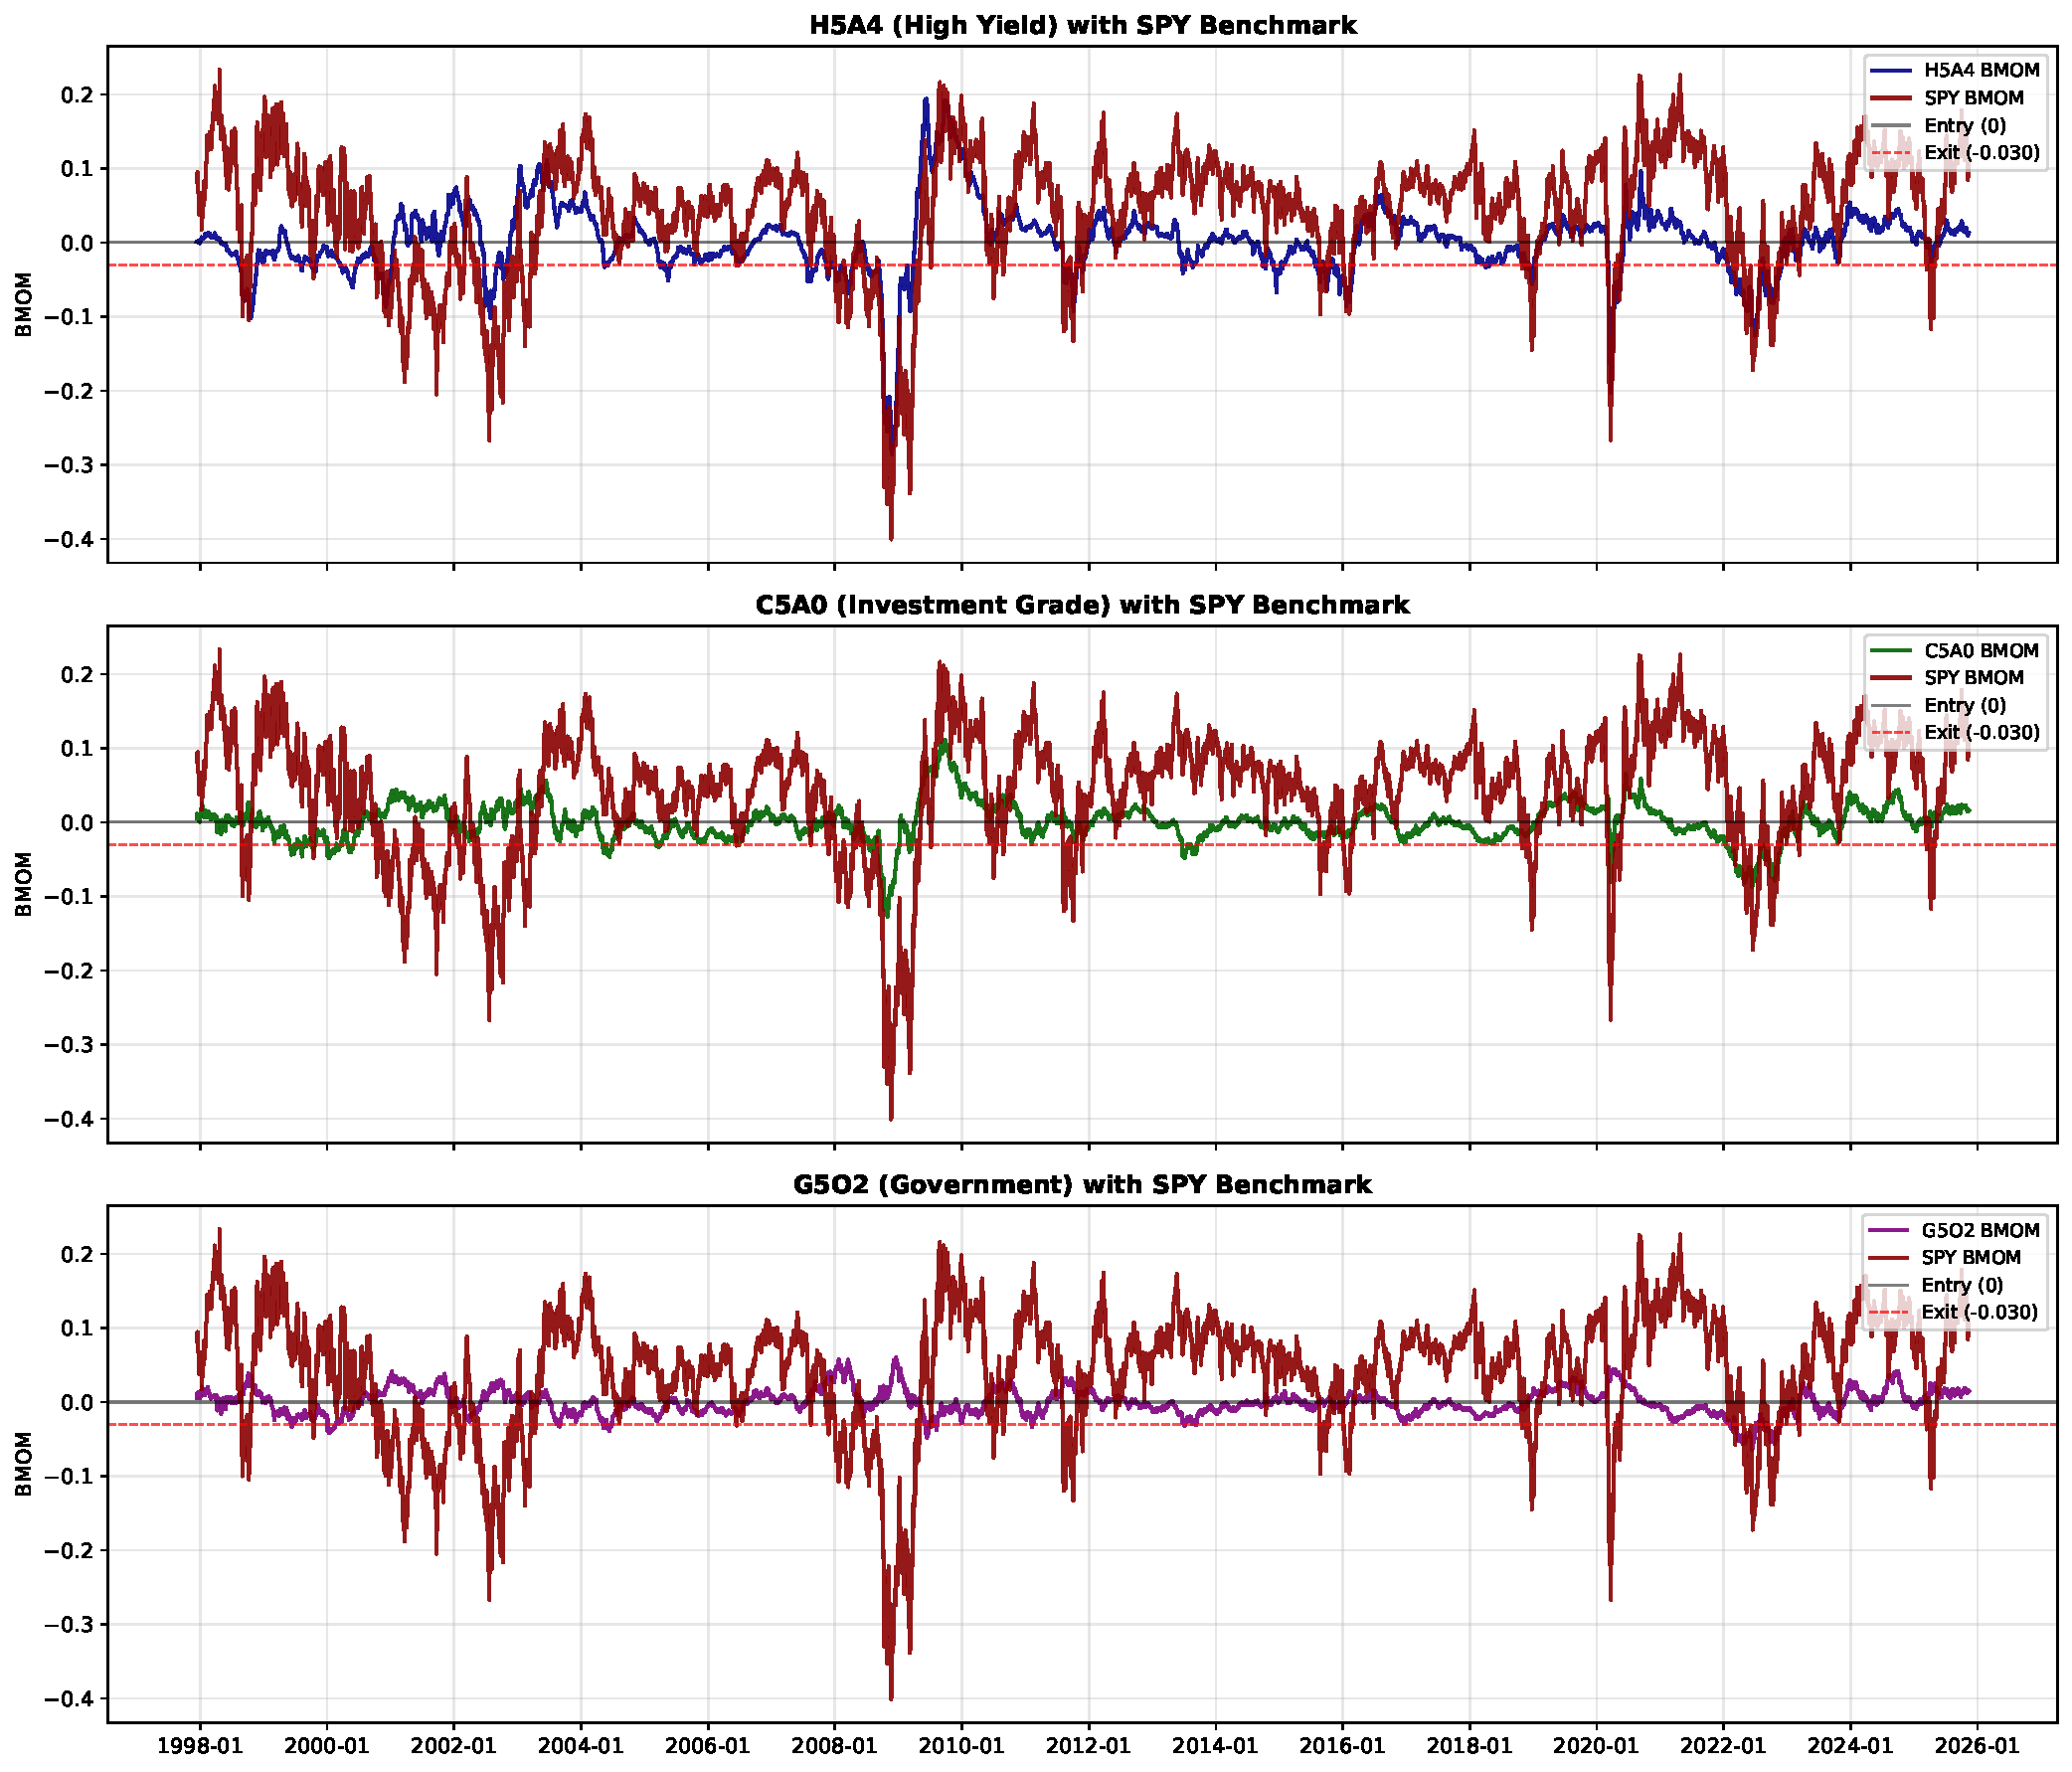
\includegraphics[width=\textwidth]{../PDFs/fig_bmom_timeseries.pdf}
    \caption{BMOM indicators for fixed income assets over time with SPY benchmark overlay. Each panel shows the asset-level BMOM (H5A4, C5A0, G5O2) alongside SPY BMOM, demonstrating the cross-asset momentum filtering framework. Horizontal lines indicate entry threshold (0) and exit threshold ($-0.03$).}
    \label{fig:bmom_timeseries}
\end{figure}

\textbf{Rationale}

Figure 1 reveals a critical pattern: the largest drawdowns in fixed income assets consistently overlap with periods of SPY BMOM deterioration. The 2008 financial crisis, 2020 COVID selloff, and 2022 interest rate shock all exhibit simultaneous weakness across both the fixed income assets and SPY, confirming that systemic drawdowns manifest as dual deterioration rather than isolated asset-class stress. This observation validates the dual-weakness filter as a systemic risk detector. When both asset and benchmark BMOMs cross below the threshold, the strategy exits during the confirmation phase of broad market stress, before drawdowns fully develop. Conversely, periods when fixed income BMOM weakens while SPY remains resilient typically represent idiosyncratic volatility, technical supply-demand imbalances, or sector-specific events that do not warrant defensive positioning. By requiring cross-asset confirmation, the strategy systematically avoids the most severe drawdowns while maintaining exposure during isolated volatility.

The use of SPY as a universal benchmark exploits the equity-credit lead-lag relationship observed in financial markets. Equity markets are highly liquid and rapidly incorporate information about corporate fundamentals and macroeconomic conditions. Credit markets, particularly corporate bonds, trade less frequently and can exhibit delayed price adjustment due to lower liquidity, institutional constraints, and over-the-counter market structure. This creates an informational advantage: equity weakness often precedes credit spread widening by hours or days.

For credit-sensitive assets (H5A4 and C5A0), requiring dual weakness (both asset BMOM and SPY BMOM below threshold) captures deteriorating conditions while they are still developing. When SPY crosses below the $-0.03$ threshold, it signals declining corporate health or risk appetite that should eventually manifest in wider credit spreads. If the fixed income asset's BMOM is also weak, this confirms the credit market is beginning to reflect the same stress. The strategy exits during this confirmation phase, using SPY's leading signal rather than waiting for credit prices to fully adjust.

For government bonds (G5O2), the dual requirement filters for rare periods of simultaneous equity and Treasury weakness. While Treasuries typically benefit from flight-to-quality flows during equity sell-offs, periods when both SPY and G5O2 show momentum deterioration indicate systemic stress conditions (such as rising rate regimes, stagflation concerns, or broad deleveraging) that warrant defensive positioning.

The cross-below detection mechanism (rather than static threshold evaluation) identifies momentum deterioration in real time. The uniform $-0.03$ threshold provides a consistent definition of momentum weakness across all assets, creating a unified framework for risk-off detection across the fixed income portfolio.

\subsection{Strategy 2: Drawdown Differential Override}

\textbf{Motivation}

While Strategy 1 provides a robust foundation for tactical allocation, asset-level analysis revealed opportunities for performance enhancement. Comparing Strategy 1 to buy-and-hold across the three assets showed:

\begin{itemize}
    \item \textbf{H5A4 (High Yield)}: Strategy 1 achieved 0.87\% annualized return with 0.24 Sharpe
    \item \textbf{C5A0 (Investment Grade)}: Strategy 1 achieved 0.54\% return with 0.18 Sharpe
    \item \textbf{G5O2 (Government)}: Strategy 1 achieved $-0.42\%$ return with $-0.14$ Sharpe
\end{itemize}

These results indicated that Strategy 1's tactical signals successfully avoided losses in credit-sensitive assets (H5A4, C5A0) but could benefit from a mechanism to remain invested during periods when the momentum-based signals were proving effective.

\textbf{Implementation}

Strategy 2 introduces an asset-level drawdown differential override applied independently to each asset. For each asset $i$, the strategy monitors:

\begin{equation}
\text{DD}_{\text{diff},i}(t) = \text{DD}_{\text{S1},i}(t) - \text{DD}_{\text{BH},i}(t)
\end{equation}

where $\text{DD}_{\text{S1},i}$ is the drawdown of Strategy 1 for asset $i$ and $\text{DD}_{\text{BH},i}$ is the buy-and-hold drawdown.

Since drawdowns are zero at equity peaks and negative during losses, the differential measures relative performance. For example, if Strategy 1 has a $-5\%$ drawdown while buy-and-hold has a $-20\%$ drawdown, the differential is $(-0.05) - (-0.20) = +0.15$. When $\text{DD}_{\text{diff},i} > 0.10$, Strategy 1's drawdown is more than 10 percentage points less severe than buy-and-hold, indicating the tactical signals are successfully avoiding losses.

\textbf{State Machine Architecture}

The override employs a regime-based state machine to capitalize on outperformance while preventing whipsaw:

\begin{enumerate}
    \item \textbf{Regime Identification}: Each time DD$_{\text{diff},i}$ crosses above 0.10, a new override regime begins and receives a unique identifier
    \item \textbf{Override Activation}: The signal is immediately forced to long (Signal = 1) when the threshold is crossed
    \item \textbf{Regime Persistence}: The long position is maintained throughout the entire override regime, even if DD$_{\text{diff},i}$ subsequently falls below 0.10
    \item \textbf{Strategic Exit}: The override regime only ends when Strategy 1 naturally signals long (Strategy 1 Signal = 1), ensuring the exit occurs when the underlying momentum logic confirms continued strength rather than forcing a transition to flat
\end{enumerate}

This architecture prevents the strategy from exiting positions prematurely when its risk management framework is demonstrably outperforming passive exposure. The state machine exit condition ensures alignment between the override and the underlying Strategy 1 signal, avoiding situations where the override would force a flat position immediately after deactivating.

\textbf{Results}

The drawdown differential override significantly improved performance across credit-sensitive assets:

\begin{itemize}
    \item \textbf{H5A4}: Sharpe increased from 0.24 to 0.28 (+16.7\%), with return improving from 0.87\% to 1.2\%
    \item \textbf{C5A0}: Sharpe increased from 0.18 to 0.29 (+61.1\%), with return improving from 0.54\% to 0.90\%
    \item \textbf{G5O2}: No change (Sharpe remained at $-0.14$), indicating rare override activation for duration-focused assets
\end{itemize}

The substantial improvement in C5A0 demonstrates the override's effectiveness in capturing outperformance during periods when tactical signals successfully navigate credit cycles.

\subsection{Proportional Linear Allocation}

Multiple allocation methodologies were evaluated during the research process, including equal weight, regime-based, and proportional approaches. Proportional linear allocation demonstrated superior risk-adjusted performance by dynamically sizing positions based on momentum signal strength, and was therefore selected for the final implementation.

\textbf{Allocation Formula}

The proportional linear framework calculates portfolio weights based on momentum-adjusted scores for each asset:

\begin{equation}
\text{Score}_i(t) = \max(0, \text{BMOM}_i(t)) \times \text{Signal}_i(t)
\end{equation}

where Signal$_i$(t) is the Strategy 2 output (0 or 1). The score isolates positive momentum (negative BMOM values are set to zero) and zeros out assets with flat signals. Raw weights are then computed as:

\begin{equation}
w_i^{\text{raw}} = \frac{\text{Score}_i}{\sum_j \text{Score}_j} \times 0.95
\end{equation}

with the remaining 5\% allocated to cash as a liquidity buffer during active periods.

\subsubsection{Weight Calculation Process}

The allocation logic follows a sequential constraint enforcement process:

\begin{enumerate}
    \item \textbf{Defensive Mode Check}: If all scores equal zero (all signals flat or negative momentum), allocate 10\% to cash and 90\% to G5O2 (government bonds)

    \item \textbf{Proportional Allocation}: Compute raw weights proportional to scores, normalized to 95\% total exposure

    \item \textbf{Minimum Position Enforcement}: For each active asset with raw weight below 5\%, increase to 5\% minimum and proportionally reduce other active assets to maintain 95\% total

    \item \textbf{High Yield Cap}: If H5A4 weight exceeds 12\%, cap at 12\% and redistribute excess to C5A0 (if active), then G5O2 (if active), otherwise to cash
\end{enumerate}

This sequential process ensures all portfolio constraints are satisfied while preserving the core principle that stronger momentum signals receive larger allocations.

\subsubsection{Portfolio Constraints}

Three critical constraints govern the final weights:

\begin{itemize}
    \item \textbf{High Yield Cap (12\%)}: Limits H5A4 exposure to manage credit concentration risk, a requirement from Regentfund portfolio guidelines

    \item \textbf{Minimum Allocation (5\%)}: Prevents trivial positions that lack meaningful portfolio impact while incurring full transaction costs

    \item \textbf{Defensive Positioning (10/90)}: When all signals turn flat, the strategy shifts to a conservative stance with minimal cash drag and maximum duration protection via government bonds
\end{itemize}

The proportional linear approach outperformed alternative allocation schemes by incorporating signal strength information (unlike equal weight) while maintaining simplicity and avoiding parameter-heavy regime classification systems.

\begin{figure}[H]
    \centering
    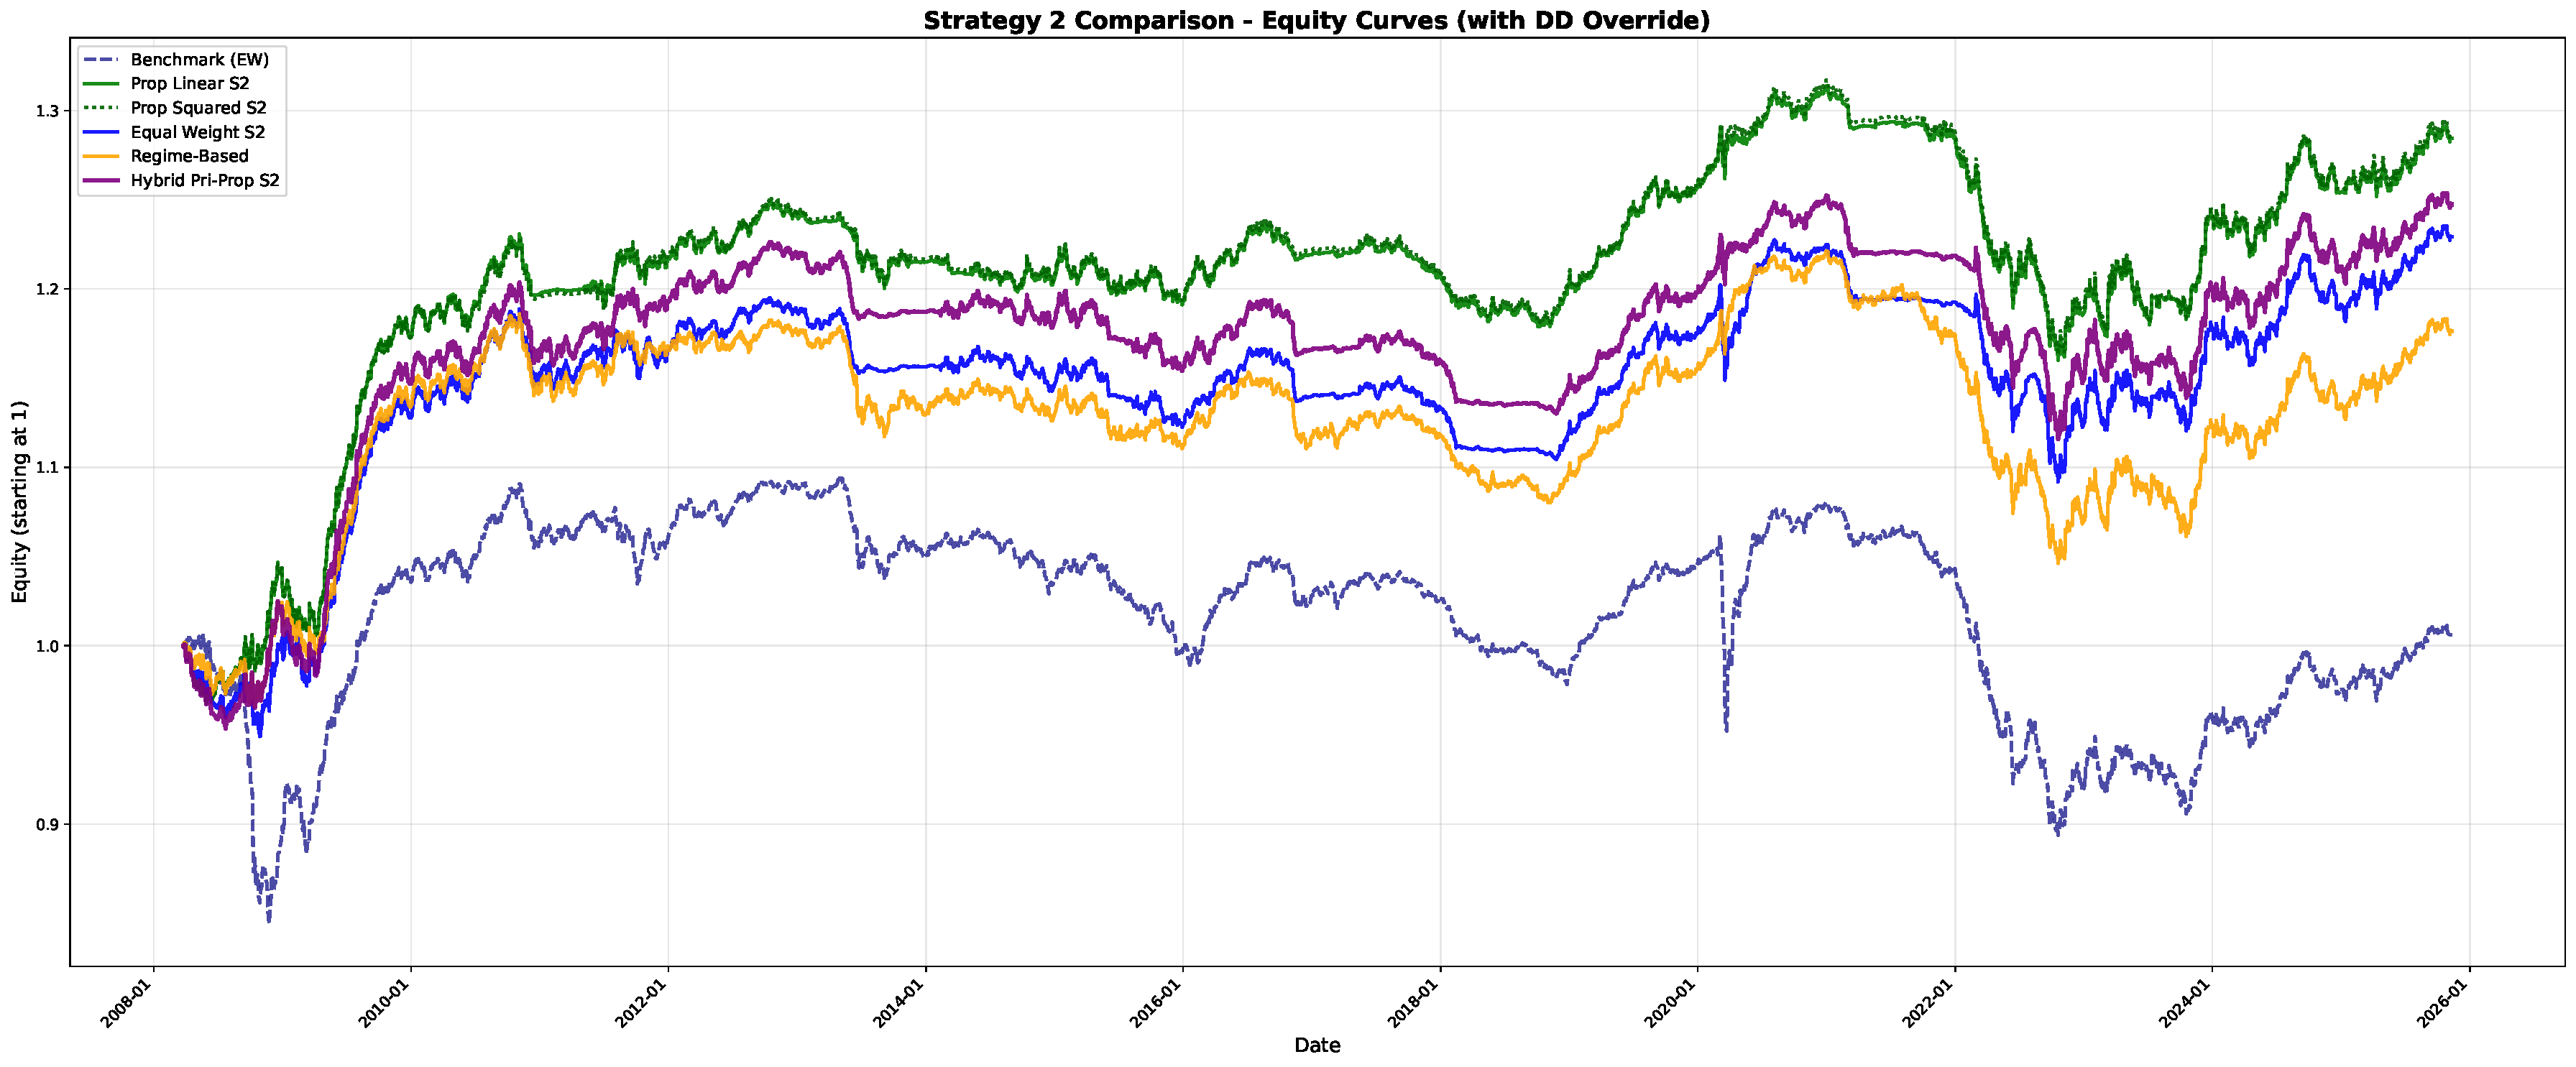
\includegraphics[width=\textwidth]{../PDFs/fig_equity_curves_strat2.pdf}
    \caption{Equity curve comparison across allocation methodologies (Proportional Linear, Equal Weight, Regime-Based), demonstrating the superior risk-adjusted performance of the proportional linear approach.}
    \label{fig:allocation_comparison}
\end{figure}

\newpage
\section{Implementation: Monthly Rebalancing Strategy}

\subsection{Rebalancing Framework}

The final implementation adapts the proportional linear allocation framework to Regentfund's operational constraint of monthly portfolio rebalancing. The Regentfund Fixed Income Portfolio executes trades on a monthly schedule, with the specific day of the month determined by portfolio managers based on operational considerations. The strategy is designed to function within this execution cadence.

\subsection{Risk-Triggered Rebalancing}

Given the monthly trading constraint, the strategy implements a dual-trigger approach to balance operational requirements with tactical risk management:

\begin{enumerate}
    \item \textbf{Scheduled Monthly Rebalancing}: Portfolio weights are recalculated and executed on the designated monthly trading date. Target weights are determined using the proportional linear allocation framework with all constraints (12\% HY cap, 5\% minimums, defensive positioning) applied.

    \item \textbf{Risk-Triggered Rebalancing}: When any asset's Strategy 2 signal transitions to 0 (flat), the strategy immediately rebalances without waiting for the next scheduled date. Weights are recalculated with the flat asset receiving zero allocation and remaining active assets reweighted proportionally. If all asset signals turn flat simultaneously, the portfolio shifts to full defensive mode (10\% cash, 90\% government bonds).
\end{enumerate}

Between rebalancing events, portfolio weights remain at their most recently calculated allocation and drift with market movements. The risk-triggered override addresses the primary limitation of monthly rebalancing by allowing immediate portfolio adjustment when Strategy 1's exit conditions (cross-below + Mom$_{240}$ < 0) are met for any asset. This preserves the tactical risk management capabilities demonstrated in Strategy 2's asset-level results while respecting Regentfund's monthly trading schedule.

\newpage
\section{Results and Performance}

\subsection{Strategy Evolution Performance}

The progression from Strategy 1 to Strategy 2 demonstrates the effectiveness of the drawdown differential override across individual assets:

\begin{table}[H]
\centering
\begin{tabular}{lccc}
\toprule
Asset & Strategy 1 Sharpe & Strategy 2 Sharpe & Improvement \\
\midrule
H5A4 (High Yield) & 0.24 & 0.28 & +16.7\% \\
C5A0 (Investment Grade) & 0.18 & 0.29 & +61.1\% \\
G5O2 (Government) & $-0.14$ & $-0.14$ & 0.0\% \\
\bottomrule
\end{tabular}
\caption{Asset-level performance improvement from Strategy 2 override}
\end{table}

The substantial improvement in C5A0 (investment grade credit) highlights the override's effectiveness in credit-sensitive markets, where the tactical signals successfully navigated credit cycle dynamics. The lack of improvement in G5O2 reflects the difficulty of timing duration exposure through momentum signals alone during the sample period.

\subsection{Final Strategy Metrics}

Transitioning from asset-level signals to portfolio construction introduced proportional linear allocation with constraints. Strategy 3 implemented daily weight monitoring with a 5\% turnover threshold to reduce transaction costs while maintaining tactical responsiveness:

\begin{table}[H]
\centering
\begin{tabular}{lcc}
\toprule
Metric & Strategy 3 & Monthly Strategy \\
\midrule
Annualized Return & 1.07\% & 0.77\% \\
Annualized Volatility & 2.95\% & 2.97\% \\
Sharpe Ratio & 0.36 & 0.26 \\
Max Drawdown & $-11.71\%$ & $-11.99\%$ \\
Win Rate & 50.83\% & 51.05\% \\
Rebalance Days & 939 & 602 \\
Trades per Month & 2.79 & 1.79 \\
\bottomrule
\end{tabular}
\caption{Portfolio-level performance comparison}
\end{table}

\textbf{Implementation Trade-offs}

Strategy 3's daily monitoring with turnover filtering achieved superior risk-adjusted returns (Sharpe 0.36) by rebalancing approximately 2.79 times per month when momentum signals or constraint violations warranted adjustment. The Monthly Strategy, constrained by Regentfund's operational requirement of monthly execution, reduced trading frequency to 1.79 times per month, resulting in lower performance (Sharpe 0.26) but meeting institutional implementation requirements.

The risk-triggered rebalancing mechanism preserved some tactical responsiveness within the monthly constraint: the 1.79 trades per month reflects scheduled monthly rebalances plus occasional mid-month defensive repositioning when asset signals turned flat. The similar win rates between strategies (51.05\% vs 50.83\%) suggests that reduced rebalancing frequency maintained tactical effectiveness while potentially avoiding some whipsaw trades.

The final Monthly Strategy represents the implementable version of the framework, sacrificing some performance for operational feasibility while maintaining the core tactical allocation logic through risk-triggered overrides.

\begin{figure}[H]
    \centering
    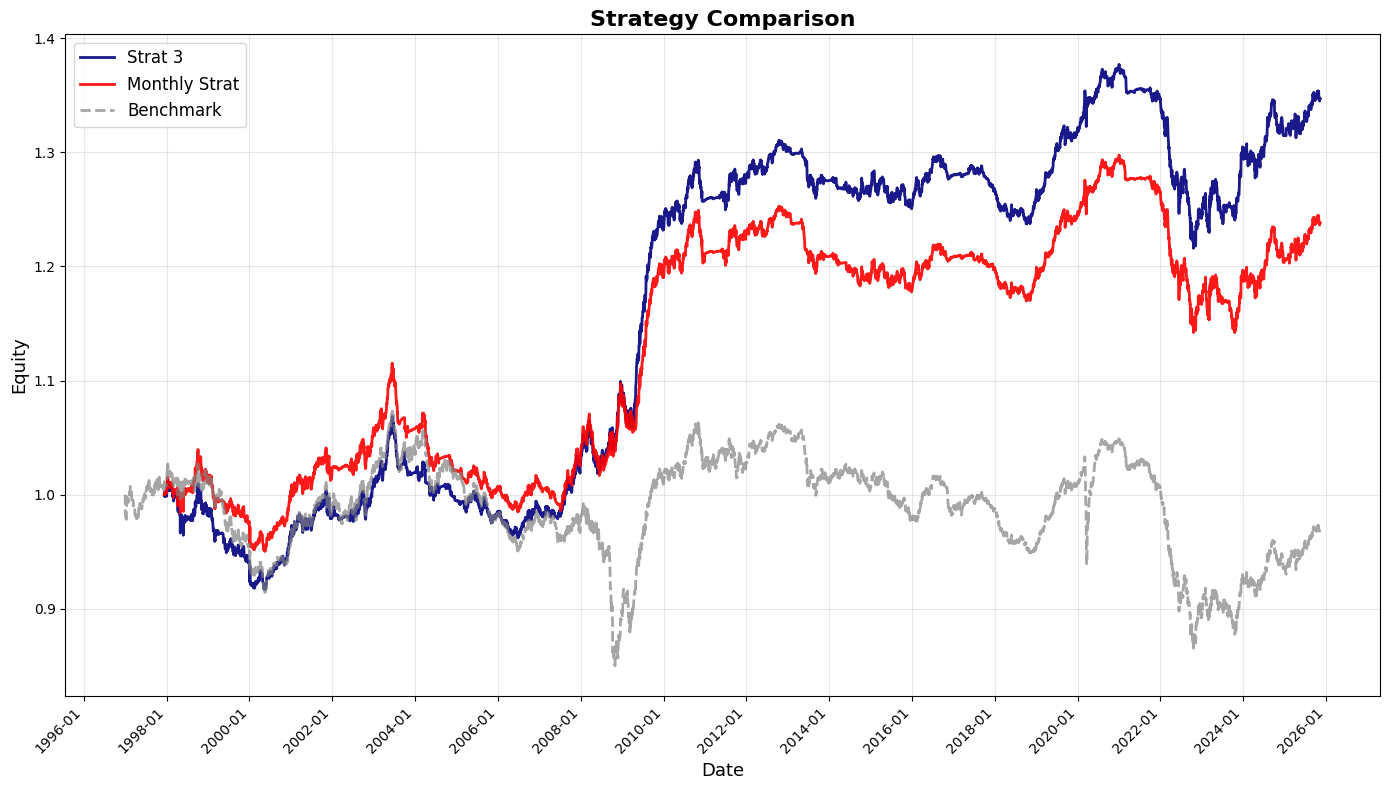
\includegraphics[width=\textwidth]{../PDFs/Regentfund_Equity_Curve.png}
    \caption{Equity curve comparison showing Strategy 3, Monthly Strategy, and Regentfund's baseline static allocation (66.5\% IG, 9.5\% HY, 19.5\% Gov, 5\% Cash) over the full sample period. Both tactical strategies substantially outperform the static benchmark, with the Monthly Strategy delivering consistent returns while respecting operational trading constraints.}
    \label{fig:final_equity_curve}
\end{figure}

\newpage
\section{Conclusion}

This whitepaper presents a comprehensive tactical asset allocation framework designed specifically for the Regentfund Fixed Income Portfolio. The Monthly Strategy delivers a ready-to-implement solution that respects operational constraints (monthly trading schedule, 12\% high yield cap) while maintaining tactical risk management capabilities through momentum-based signal generation and risk-triggered rebalancing.

The research process identified Strategy 2's drawdown differential override as the critical innovation, particularly for credit-sensitive assets where the mechanism achieved substantial performance improvements (C5A0 Sharpe increased 61\% from 0.18 to 0.29). Rather than simply avoiding losses, the override capitalizes on periods when tactical signals demonstrably outperform passive exposure, forcing positions to remain long until the underlying momentum logic confirms exit timing. This state machine architecture prevents premature exits and aligns override exits with natural signal strength.

The framework's risk management approach combines multiple defensive layers: cross-asset benchmark filtering identifies broad market stress rather than idiosyncratic volatility, the Mom$_{240}$ filter prevents exits during temporary pullbacks within long-term uptrends, and dual-trigger rebalancing preserves tactical responsiveness within monthly operational constraints. When all signals turn flat, the strategy shifts to explicit defensive positioning (10\% cash, 90\% government bonds), providing systematic tail risk management.

The Monthly Strategy achieves a 0.26 Sharpe ratio with 0.77\% annualized return and $-11.99\%$ maximum drawdown while executing approximately 1.79 trades per month. The performance gap relative to Strategy 3 (0.36 Sharpe, 1.07\% return) reflects Regentfund's monthly trading constraint rather than framework design limitations. The risk-triggered rebalancing mechanism successfully preserves defensive capabilities, allowing immediate repositioning when Strategy 1 exit conditions are met for any asset.

Future research could enhance the framework through two directions: (1) lasso regression to optimize the monthly rebalancing logic by selecting the most predictive momentum features and reducing overfitting risk, and (2) machine learning-based regime classification to improve the identification of market states (risk-on, defensive, crisis) and enable more nuanced allocation adjustments across regimes.

The Monthly Strategy is recommended for implementation in the Regentfund Fixed Income Portfolio. The framework provides systematic, rules-based tactical allocation with demonstrated risk management effectiveness across multiple market environments while meeting all operational and portfolio constraint requirements.

% Appendix (optional)
% \newpage
% \appendix
% \section{Parameter Summary}
% TO BE FILLED

\end{document}
